\documentclass{standalone}
\usepackage[dvipsnames,svgnames,x11names]{xcolor}
\usepackage{tikz}
\usepackage{pgfplots}
\pgfplotsset{compat = 1.12}
\usepackage{../thesismath}
\begin{document}
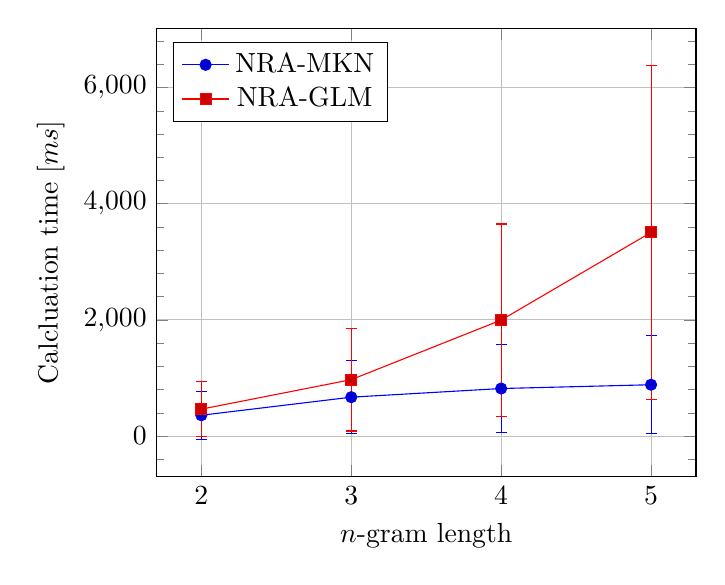
\begin{tikzpicture}[baseline]

\begin{axis}[
  xlabel = {$n$-gram length},
  xtick = {2, ..., 5},
  ylabel = {Calcluation time [$m s$]},
  minor y tick num = 4,
  grid = major,
  legend entries = {{NRA-MKN}, {NRA-GLM}},
  legend pos = north west,
]

% over 100 test sequences on my own machine

% NRA-MKN
\addplot+[
  error bars/.cd,
  y dir = both,
  y explicit,
] table [y error = us_error] {
  n us       us_error
  2  358.575  412.311
  3  669.639  626.573
  4  818.547  762.427
  5  883.680  844.083
};

% NRA-GLM
\addplot+[
  error bars/.cd,
  y dir = both,
  y explicit,
] table [y error = us_error] {
  n us       us_error
  2  463.283  474.245
  3  970.982  884.137
  4 1996.918 1654.564
  5 3506.086 2871.907
};

\end{axis}

\end{tikzpicture}
\end{document}
